\subsection{Overdrive and Distortion}\label{sec:overdrive} 

The distortion effects changes the sound of the played instrument by increasing the gain and thereby the sound changes due to the clipping effect.
The clipping effect is a way of changing the waveform when an amplifier is overdriven; forcing it to deliver an output that is higher than its maximum capability. 
The part of the waveform where the amplifier is asked to get a value higher than its maximum capacity gets the maximum value the amplifier can give. It means that all the parts of the waveform where the amplifier is pushed more than its capacity will have the same amplitude. The signal is then 'clipped'. An illustration of this effect is shown in \autoref{fig:clipping1} \citep{distortion_clipping1}.\\

\begin{figure} [htbp]
	\centering
  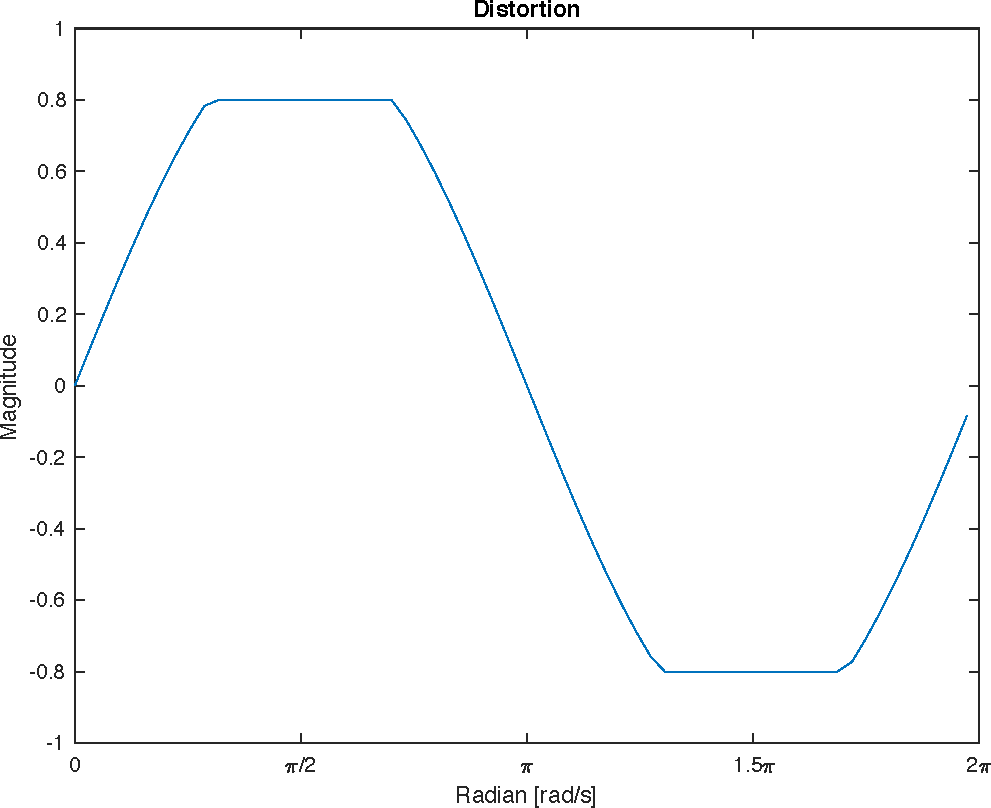
\includegraphics[width=0.9\textwidth]{clippingeffect.pdf}
  \caption{Illustration showing the effect of clipping, a consequence of the overdrive or distortion effect.}
  \label{fig:clipping1}
\end{figure} \citep{distortion_clipping1}


The consequences in the frequency domain are that the clipping effect creates more harmonics than the signal without the clipping effect \citep{distortion_harmonics}. 
The clipping effect in digital signal processing happens when the amplitude is limited by storage capacity of the used device and if during the processing the amplitude surpasses this limit, clipping happens because the value is then set to the maximum amplitude that can be handled digitally \citep{distortion_digital}. The maximum amplitude that can be handled is determined by the number of bits the system uses. The maximum number for a \SI{16}{\bit}  signed integers system is $\frac{2^{16}}{2} = \SI{32768}{\cdot}$ which means that if a value has an amplitude higher than this number the clipping effect occurs \citep{distortion_digitalcalc}. 
Digital distortion and overdrive are hard to design to a specific sound, compared with the analog distortion and overdrive effects. When designing a digital distortion effect, it can be done by measuring on an analog distortion effect and then reproduce the characteristics of the analog effect. The analog distortion or overdrive effects are often made by using the nonlinearity of the saturation area of either a diode or a transistor \citep{CCRMA}. 

Effects of hard and soft clipping on the waveforms are shown in \autoref{fig:clipping2}. Hard clipping changes the signal more than the soft clipping, soft clipping tends to soften higher amplitudes than hard clipping which creates a cleaner sound \citep{distortion_softhardclipping}. Hard clipping adds more harmonics than soft clipping \citep{distortion_harmonics}. 

In the previous paragraphs, distortion and overdrive has been explained as if they are the same effects. In fact, there is a small difference between the two. Distortion changes the original signal more than overdrive which means that distortion will generate more extra harmonics than overdrive and their amplitude tend to be higher. Overdrive effect has "cleaner" consequences on the final signal than distortion. Overdrive is often assigned to soft clipping while distortion is assigned to hard clipping \citep{distortion_difference}.


\begin{figure} [htbp]
	\centering
  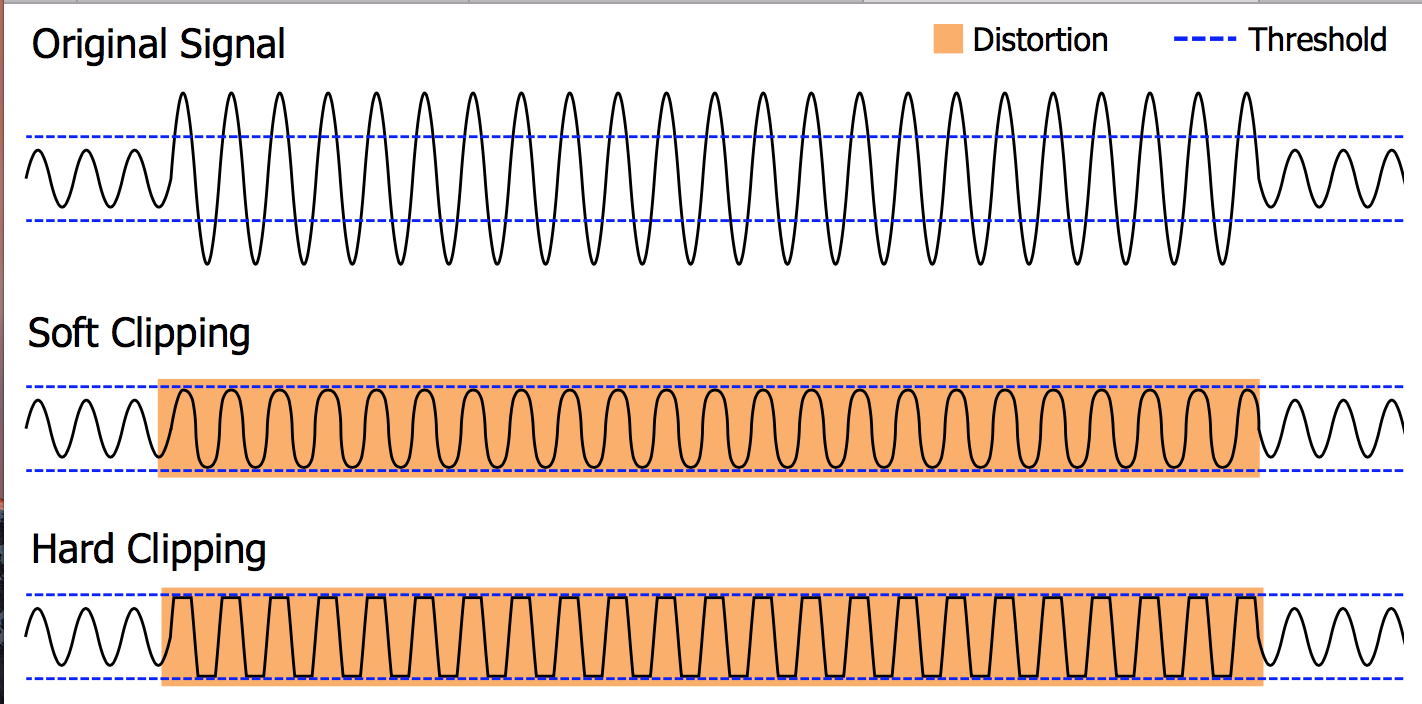
\includegraphics[width=0.7\textwidth]{softhardclipping.png}
  \caption{Photo showing the effect of hard and soft clipping, a consequence of the overdrive or distortion effect \citep{distortion_difference}.}
  \label{fig:clipping2}
\end{figure}

A simple block diagram is shown in \autoref{fig:overdrive_block}.

\begin{figure} [htbp]
	\centering
\begin{picture}(0,0)%
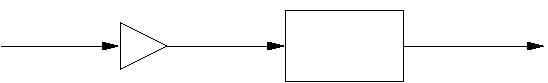
\includegraphics{overdrive_block.pdf}%
\end{picture}%
\setlength{\unitlength}{4144sp}%
%
\begingroup\makeatletter\ifx\SetFigFont\undefined%
\gdef\SetFigFont#1#2#3#4#5{%
  \reset@font\fontsize{#1}{#2pt}%
  \fontfamily{#3}\fontseries{#4}\fontshape{#5}%
  \selectfont}%
\fi\endgroup%
\begin{picture}(4167,627)(-374,-703)
\put(901,-241){$Gain$}%
\put(1846,-466){$Clipping$}%
\put(-359,-286){$Input$}%
\put(2881,-286){$Output$}%
\end{picture}%
  \caption{Photo showing the effect of hard and soft clipping, a consequence of the overdrive or distortion effect.}
  \label{fig:overdrive_block}
\end{figure}

The above block diagram \autoref{fig:overdrive_block} shows a simple block diagram of distortion and overdrive. As described the only difference is the clipping softness of the clipping block. 